\documentclass[10pt,letterpaper]{article}
\RequirePackage{amsthm,amssymb,amsmath,graphicx}
\RequirePackage[top=2cm, bottom=2cm, left=2.5cm, right=3cm]{geometry}
\usepackage{caption}
\usepackage{subcaption}
\usepackage[pagebackref=false,colorlinks,linkcolor=black,citecolor=magenta]{hyperref}
\RequirePackage{MnSymbol}
\newcommand{\eqn}[2]{
\begin{equation}
\begin{split}
#1
\label{#2}
\end{split}
\end{equation}
}
%%%%%%%%%%%%%

%       \eqn{
%       x=x^2
%       }{label}

%%%%%%%%%%%%%
\newcommand{\feqn}[2]{
\begin{tcolorbox}[width=7in, colback=white]
\begin{equation}
\begin{split}
#1
\label{#2}
\end{split}
\end{equation}
\end{tcolorbox}
}
%%%%%%%%%%%%%%%
\newcommand{\hl}{
\begin{center}
\line(1,0){450}
\end{center}}
\setlength{\parindent}{0pt}
\newcommand{\nl}{\newline\newline}
\newcommand{\pic}[1]{
\begin{center}
\includegraphics[width=130mm]{#1}
\end{center}
}
%\settextfont{B Nazanin}
\usepackage{lipsum}
\newtheorem{theorem}{Theorem}
\begin{document}
\Large
\begin{center}
The solution of assignment \#10 of the \textbf{ComNet} course
\end{center}
\hl
Q1) a. Confidentiality is keeping the message secret such that no intruder can understand the data. In contrast, end-point authentication refers to a scheme where each of both sides of a transmission can confirm the other side's identity and to make sure they `really' are who they pretend to be.
\newline\newline
b. Since the protocol is not kept from the intruder, the legitimate sender and receiver must agree upon some secret information that is not revealed to any third-party user.
\newline\newline
Q2) a \& b)
\begin{center}
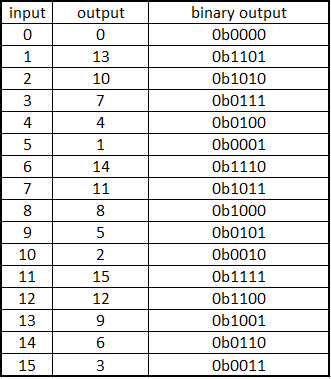
\includegraphics[width=70mm]{Table_10.png}
\end{center}
As it can be seen, the outputs are unique.

Another way for proving the uniqueness, is the following deduction
$$
x\equiv y\mod 16\iff 13x\equiv 13y\mod 16
$$
c. The transition flow in hexadecimal representation is
\begin{center}
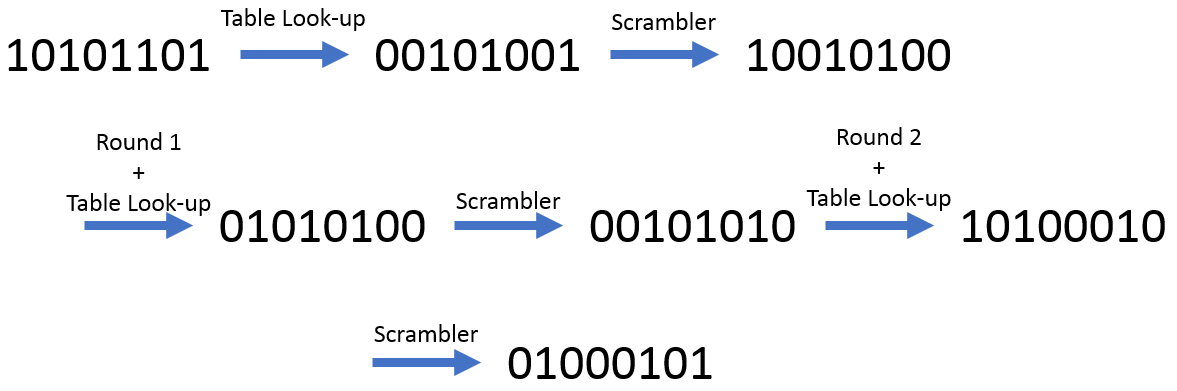
\includegraphics[width=100mm]{Trans.png}
\end{center}
d. Similar to the alternative proof in part a, any number coprime to 16 can be replaced instead of 13.
\newline\newline
Q3) The intruder, having the hash output at hand, can find out the number of digits equal to $0,1,2,\cdots ,9$, but does not know their arrangement. The best he can do, is to arrange a digit of each of 1, 2, 4, 5 and 6 and three digits of 3 randomly. He ends up with a total of 
$
{8!\over 1!\times1!\times3!\times1!\times1!\times1!}=6720
$
 different cases and his probability of detection becomes $1\over 6720$.
\newline\newline
Q4) The little Fermat's theorem implies
\begin{theorem}
$$
a^p\equiv a\mod p\quad,\quad p\text{ is prime}
$$
which reduces to
$$
a^{p-1}\equiv 1\mod p\quad,\quad p\text{ is prime}
$$
when $\gcd(a,p)=1$
\end{theorem}
also we use another theorem to conclude the final answer.
\begin{theorem}
$$
a\equiv b\mod p\quad,\quad a\equiv b\mod q\implies a\equiv b\mod pq\quad,\quad p\text{ and }q\text{ are prime}
$$
\end{theorem}
Alice's encryption:
\eqn{
c=m^e\mod n=2^{13}\mod 77=8192\mod 77=30
}{}
Bob's decryption:
\eqn{
\hat m=c^d\mod 77=30^{37}\mod 77
}{}
We know that
\eqn{
&30^6\equiv 1\mod 7
\\&
30^{10}\equiv 1\mod 11
}{}
therefore
\eqn{
&30^{36}\equiv 1\mod 7
\\&
30^{30}\equiv 1\mod 11
}{}
and
\eqn{
&30^{37}\equiv 30\equiv2\mod 7
\\&
30^{37}\equiv 30^7\equiv (-3)^7
\\&
\equiv -3\times 27^2
\\&
\equiv -3\times 5^2
\\&
\equiv -75
\\&
\equiv 2\mod 11
}{}
since
\eqn{
&30^{37}\equiv 2\mod 7
\\&30^{37}\equiv 2\mod 11
}{}
we conclude that
$$
30^{37}\equiv 2\mod 77
$$
and therefore, Bob can decrypt Alice's message uniquely.

Jake's decryption:
\eqn{
\hat m=c^d\mod 77=30^{97}\mod 77
}{}
We know that
\eqn{
&30^{6}\equiv 1\mod 7
\\&
30^{10}\equiv 1\mod 11
}{}
therefore
\eqn{
&30^{96}\equiv 1\mod 7
\\&
30^{90}\equiv 1\mod 11
}{}
and
\eqn{
&30^{37}\equiv 30\equiv2\mod 7
\\&
30^{97}\equiv 30^7\equiv (-3)^7
\\&
\equiv -3\times 27^2
\\&
\equiv -3\times 5^2
\\&
\equiv -75
\\&
\equiv 2\mod 11
}{}
since
\eqn{
&30^{97}\equiv 2\mod 7
\\&30^{97}\equiv 2\mod 11
}{}
we conclude that
$$
30^{97}\equiv 2\mod 77
$$
and therefore, Jake can decrypt Alice's message uniquely.
\newline\newline
b. To show (4)$\implies$(3), assume by contrary that $\gcd(e,z)\ne 1$. Then, $x\in \Bbb Z$ and $x>1$ exists such that $\gcd(e,z)=x$ which means that $x|e$ and $x|z$. Since condition (4) holds, we have
\eqn{
z|ed-1&\implies x|ed-1
\\&
\implies x|xq-1\quad,\quad\text{for some }q\in\Bbb Z
\\&
\implies x|-1
}{}
which is a contradiction. Hence (3) must hold in order for (4) to hold and the proof is complete $\blacksquare$
\end{document}